\documentclass[border=10pt]{standalone}
\usepackage{tikz}

\begin{document}
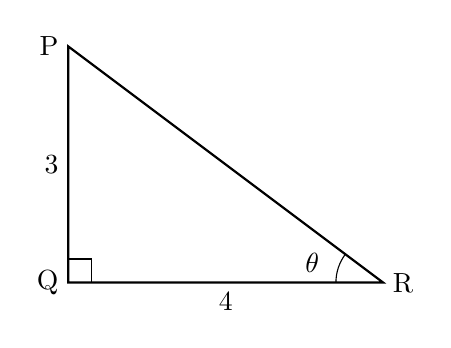
\begin{tikzpicture}[scale=1]
    % Define coordinates for the triangle
    \coordinate (Q) at (0,0);
    \coordinate (P) at (0,3);
    \coordinate (R) at (4,0);

    % Draw the sides of the triangle
    \draw[thick] (P) -- (Q) -- (R) -- cycle;

    % Draw the right-angle symbol at Q
    \draw (0,0.3) -- (0.3,0.3) -- (0.3,0);

    % Labels for the vertices
    \node[left] at (P) {P};
    \node[left] at (Q) {Q};
    \node[right] at (R) {R};

    % Length measurements
    \node[left] at (0,1.5) {3};
    \node[below] at (2,0) {4};

    % Angle arc and label for theta
    \draw (3.4,0) arc (180:143:0.6);
    \node at (3.1,0.25) {$\theta$};
\end{tikzpicture}
\end{document}
